\documentclass[border=6pt]{standalone}
% ---------------------------------------------------------------------------
% tikzpreamble.tex -- shared by main.tex and by every standalone in tikz/
% ---------------------------------------------------------------------------
\usepackage{amsmath}
\usepackage{amssymb}
\usepackage{tikz}
\usepackage{circuitikz}
\usetikzlibrary{arrows.meta,calc,positioning,decorations.pathmorphing,decorations.pathreplacing,
                decorations.markings,patterns,angles,quotes,fit,
                shapes.geometric,shapes.misc,backgrounds,intersections}

\ctikzset{bipoles/length=0.85cm}
\ctikzset{resistors/scale=0.85}
\ctikzset{capacitors/scale=0.9}

\tikzset{
  wire/.style      = {line width=0.7pt},
  dashedwire/.style= {line width=0.7pt, densely dashed},
  term/.style      = {circle, draw, line width=0.6pt, fill=white,
                      inner sep=0pt, minimum size=4.5pt},
  node dot/.style  = {circle, fill=black, inner sep=0pt, minimum size=4pt},
  boxlabel/.style  = {font=\sffamily\small},
  annot/.style     = {font=\small, align=left},
  phasor/.style    = {-{Stealth[length=3.2mm,width=2.2mm]}, line width=1.1pt},
  thinphasor/.style= {-{Stealth[length=2.6mm,width=1.8mm]}, line width=0.7pt},
  axis line/.style = {-{Stealth[length=2.6mm,width=1.8mm]}, line width=0.6pt},
  guide/.style     = {densely dashed, line width=0.4pt, gray},
}
\usepackage{siunitx}

\begin{document}
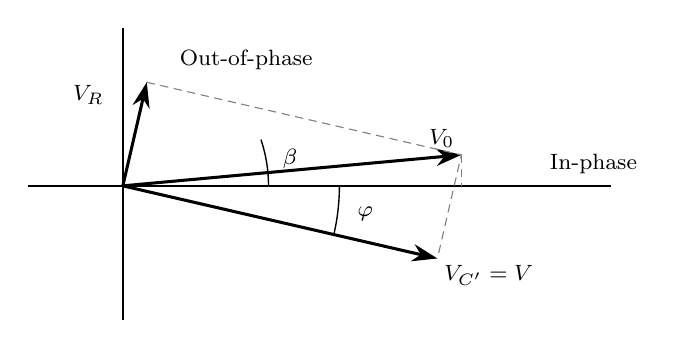
\begin{tikzpicture}[every node/.style={font=\small}]
  \draw[line width=0.5pt] (0,-1.7) -- (0,2.0);
  \draw[line width=0.5pt] (-1.2,0) -- (6.2,0);
  \node[anchor=south west,font=\footnotesize] at (0.6,1.35) {Out-of-phase};
  \node[anchor=west,font=\footnotesize] at (5.3,0.28) {In-phase};

  \coordinate (O)   at (0,0);
  \coordinate (VCp) at (-13:4.1);           % V_{C'} = V (measured)
  \coordinate (VR)  at (77:1.35);
  \coordinate (V0)  at ($(VCp)+(VR)$);

  \draw[phasor] (O) -- (VCp) node[anchor=north west,font=\footnotesize,inner sep=2pt] {$V_{C'}=V$};
  \draw[phasor] (O) -- (VR);
  \node[anchor=east,font=\footnotesize] at (-0.12,1.15) {$V_R$};
  \draw[phasor] (O) -- (V0)  node[anchor=south east,font=\footnotesize,inner sep=2pt] {$V_0$};
  \draw[guide] (VR) -- (V0) -- (VCp);
  \draw[guide] (V0) -- (V0 |- O);

  \draw[line width=0.5pt] (1.85,0) arc[start angle=0,end angle=18.5,radius=1.85];
  \node[font=\footnotesize] at (9:2.15) {$\beta$};
  \draw[line width=0.5pt] (2.75,0) arc[start angle=0,end angle=-13,radius=2.75];
  \node[font=\footnotesize] at (-6.5:3.1) {$\varphi$};
\end{tikzpicture}
\end{document}
